\ifSTANDALONE
\section{Wirkungsweise} \label{wirkungsweise}
\fi
\ifEMBED
\subsection{Wirkungsweise} \label{wirkungsweise}
\fi

\ifEMBED
    % Dieses Kapitel ist eine Zusammenarbeit der Gruppen \BLDCTeams. 
    \BLDCcollab
\fi
    
    Schrittmotoren oder auch Stepper genannt, sind Synchronmotoren, bei welchen der Rotor um einen bestimmten Winkel gedreht werden kann. So ist die Rotorposition ohne zusätzliche Sensoren bekannt. Dabei ist zu beachten, dass der Motor keine Schritte verliert, was bei Überlast geschehen kann. Da die meisten Schrittmotorensysteme Open- Loop Systeme sind, entsteht eine dauernde Positionsabweichung bei einem Schrittverlust. Grundsätzlich wird zwischen zwei Schrittmotortypen unterschieden: 
    \begin{itemize}
       	\item Permagnentmagnetmotor
       	\item Reluktanzmotor
    \end{itemize} 
    Der Permanentmagnetmotor besitzt als Rotor einen Permagnentmagneten. Beim Reluktanzmotor besteht der Rotor aus einem gezahnten Weicheisenkern. Permanentmagnetmotoren erreichen eine kleinere Schrittfrequenz, besitzen jedoch ein grösseres Drehmoment als der Reluktanzmotor. Die Kombination aus Reluktanzmotor und Permanentmagnetmotor ist ein Hybridmotor. Ein Hybridmotor verbindet die Vorteile von Reluktanz- und Permagnentmotor.
    
    Der Vollschrittbetrieb kann einphasig oder auch zweiphasig gesteuert werden. Beim einphasigen Vollschrittbetrieb sind immer zwei gegenüber liegende Pole aktiv. Beim zweiphasigen Vollschrittbetrieb werden jeweils zwei nebeneinander liegende Pole aktiv. Im Halbschrittbetrieb werden die beiden Vollschrittbetriebsarten kombiniert. So kann der Schrittwinkel halbiert werden. Zusätzlich kann der Schrittmotor mit Mikroschritten betrieben werden. Dabei folgt der Strom der sinusförmigen Referenzspannung. (Vgl. Seite \pageref{stromgesteuert})
    \begin{figure}[H]
    	\centering
    	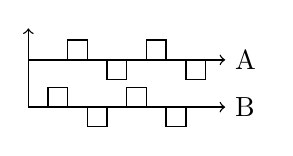
\begin{tikzpicture}
    	\draw[line width=0.5pt, ->]	(0, 0) -- (0, 1);
    	\draw[line width=0.5pt, ->]	(0, 0.6) -- (2.5, 0.6) node[right]{A};
    	\draw[line width=0.5pt, ->]	(0, 0) -- (2.5, 0) node[right]{B};
    	\draw[line width=0.5pt]    	(0.25, 0) rectangle (0.5, 0.25);
    	\draw[line width=0.5pt]    	(0.5, 0.6) rectangle (0.75, 0.85);
    	\draw[line width=0.5pt]    	(0.75, 0) rectangle (1, -0.25);
    	\draw[line width=0.5pt]    	(1, 0.6) rectangle (1.25, 0.35);
    	\draw[line width=0.5pt]    	(1.25, 0) rectangle (1.5, 0.25);
    	\draw[line width=0.5pt]    	(1.5, 0.6) rectangle (1.75, 0.85);
    	\draw[line width=0.5pt]    	(1.75, 0) rectangle (2, -0.25);
    	\draw[line width=0.5pt]    	(2, 0.6) rectangle (2.25, 0.35);
    	\end{tikzpicture}
    	\caption{Vollschritt}
    	\label{fig:vollschritt}
    \end{figure}
    
     \begin{figure}[H]
     	\centering
     	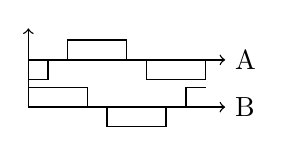
\begin{tikzpicture}
     	\draw[line width=0.5pt, ->]	(0, 0) -- (0, 1);
     	\draw[line width=0.5pt, ->]	(0, 0.6) -- (2.5, 0.6) node[right]{A};
     	\draw[line width=0.5pt, ->]	(0, 0) -- (2.5, 0) node[right]{B};
     	\draw[line width=0.5pt]    	(0,0.6) rectangle (0.25, 0.35);
     	\draw[line width=0.5pt]    	(0, 0) rectangle (0.75, 0.25);
     	\draw[line width=0.5pt]    	(0.5, 0.6) rectangle (1.25, 0.85);
     	\draw[line width=0.5pt]    	(1, 0) rectangle (1.75, -0.25);
     	\draw[line width=0.5pt]    	(1.5, 0.6) rectangle (2.25, 0.35);
     	\draw[line width=0.5pt]    	(2, 0) -- (2, 0.25);
     	\draw[line width=0.5pt]    	(2, 0.25) -- (2.25, 0.25);
     	\end{tikzpicture}
     	\caption{Halbschritt}
     	\label{fig:halbschritt}
     \end{figure}
    \begin{figure}[H]
    	\centering
    	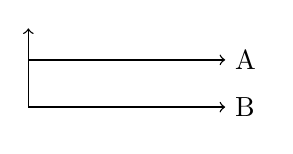
\begin{tikzpicture}
    	\draw[line width=0.5pt, ->]	(0, 0) -- (0, 1);
    	\draw[line width=0.5pt, ->]	(0, 0.6) -- (2.5, 0.6) node[right]{A};
    	\draw[line width=0.5pt, ->]	(0, 0) -- (2.5, 0) node[right]{B};
    	
    	\end{tikzpicture}
    	\caption{Mikroschritt}
    	\label{fig:mikroschritt}
    \end{figure}
    Eine Phase sind jeweils die zusammengeschalteten Statorwicklungen. Der unipolare Schrittmotor besteht aus vier Phasen. Ein Elektromagnet besteht aus zwei Phasen, welche gegenseitig gewickelt sind. So kann vermieden werden, dass der Stromfluss durch die Wicklung gedreht werden muss. Der Bipolare Schrittmotor besteht aus nur zwei Phasen. Es muss mit einer Brückenschaltung die Richtung des Stromes gedreht werden. In den meisten Anwendungen werden Bipolare Schrittmotoren verwendet, da ein bipolarer Schrittmotor ein grössseres Drehmoment erzeugt als ein gleich grosser unipolarer Schrittmotor. Die beiden Betriebsarten sind in der \autoref{fig:uniVsbi} ersichtlich. 
    \begin{figure}[H]
       	\centering
       	\includegraphics[width=12cm]{src/Bilder/uniVsbi.JPG}
       	\caption{bipolarer und unipolarer Betrieb}
       	\label{fig:uniVsbi}
    \end{figure}
    
       
    